\section{Indoor Positioning}\label{sec:analysis:indoor-positioning}

The focus of this project is not to position devices, 
and as such it was not the intention to spend time developing an entire solution for positioning devices indoors. 
Instead it was desired to find an existing product, 
that could be used to facilitate indoor positioning.
The solution should be available in the early phases of the project, 
in order to start building the system based on the solution for positioning.

As the target group of the project is consumers, 
and not businesses with big budgets, 
it is desired that the price of the technology used for indoor positioning is kept at a minimum. 
This includes the price for any device, 
that may have to be installed on each controllable device in order to position it.

It is assumed that users already own one or more devices that fit within the concept of Internet of Things, 
and are early adapters of such technology. 
However, it easy to imagine that this project can be used in an office environment, 
where employees of varying technological expertise work or in health care. 
Therefore users may have a varying degree of technological expertise, 
and it should be easy to extend the solution with new controllable devices.

Naturally the accuracy of the solution used for indoor positioning plays an important part. 
\Cref{fig:indoor-positioning:incorrect} shows the consequence of an incorrect location. 
If a lamp is estimated to be at another location that it is actually located, 
the user must point to an incorrect location in order to control the lamp.
Furthermore if the estimate is too wide, 
\ie the given area in which the lamp is located is very big, 
there is a greater risk that locations overlap. 
Overlapping locations causes a complexity, 
as it is necessary to determine which device the user desires to control, 
if he points at the overlap as visualized in \Cref{fig:indoor-positioning:overlap}.

\begin{figure}[!htb]
    \centering
    \begin{minipage}[t]{0.45\textwidth}
        \centering
        
\includegraphics[width=0.6\textwidth]{images/incorrect-positioning-estimate.png}
        \caption{Incorrect location estimate. The estimate is visualized as a striped circle. The actual location of the device is illustrated as a bulb with a circle around.}
        \label{fig:indoor-positioning:incorrect}
    \end{minipage}\qquad
    \begin{minipage}[t]{0.45\textwidth}
        \centering
        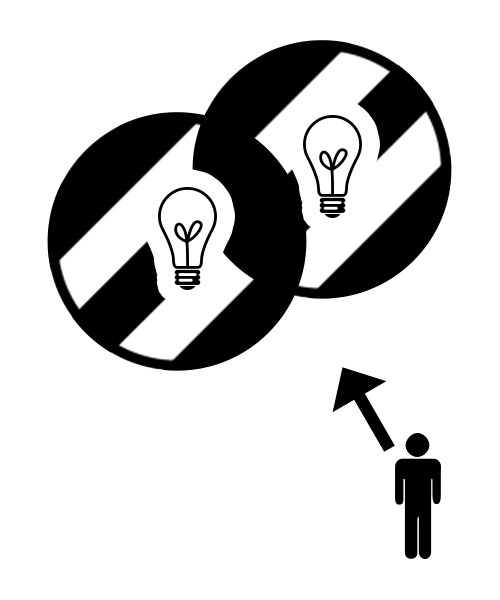
\includegraphics[width=0.6\textwidth]{images/positioning-overlap.png}
        \caption{Overlap of estimated positions. The estimates are visualized as a striped circle.}
        \label{fig:indoor-positioning:overlap}
    \end{minipage}
\end{figure}


\subsection{Analysis of Potential Existing Solutions}
This section will be an analysis of commercialized products that offer indoor location.
Only solutions intended for indoor positioning are considered.
GPS is not considered a potential solution as GPS is meant for outdoor positioning, 
and the location offered by GPS tend to have poor accuracy indoors \cite{Liu:4343996}.
Furthermore WiFi is not considered, 
as analyses have shown the accuracy of such solutions to be \SI{2}{\meter} and above \cite{Liu:4343996,jekabsons2011analysis}.
Technologies like NFC and RFID were not considered for positioning in this project either. 
Such systems only detect users when they walk by the sensors, 
and then report which sensor was activated.
We were looking for technologies that provide a more granular position of the user. 

Furthermore, we have chosen not to include solutions designed for larger buildings such as airports, malls or warehouses, 
as these does not provide solutions or setups for smaller areas such as rooms or houses. 

\Cref{tbl:indoor-positioning} shows the results of our analysis. 
\begin{table}[!htb]
    \begin{description}[style=multiline,leftmargin=2.5cm]
        \item[Product:] Estimote Beacons and Stickers \cite{estimote}
        \item[Availability:] Beacons and Stickers are shipping. SDKs available.
        \item[Technology:] iBeacon protocol.
        \item[Price:] \SI{99}[\$]{} for beacons. \SI{99}[\$]{} for \num{10} stickers, one per device to be positioned.
        \item[Ease of use:] Initial installation of beacons. Attach each sticker to device.
        \item[Accuracy:] \num{0.5}-\num{1} meter \cite{estimote:accuracy}. However the accuracy is reported to be \num{3}-\num{4} meters on average, for locations bigger than \SI{100}{\square\meter} based on an e-mail correspondence with Wojtek Borowicz from Estimote. See \Cref{appendix:estimote-accuracy}.

        \item[Product:] Pozyx \cite{pozyx}
        \item[Availability:] Available for preorder.
        \item[Technology:] Ultra-wideband (UWB).
        \item[Price:] \SI{368}[\$]{}\ for anchors. \SI{123}[\$]{} for each device to be positioned, plus supported Arduino.
        \item[Ease of use:] Initial installation of anchors. One tag for each device, plus supported Arduino. Not meant for mounting.
        \item[Accuracy:] Claimed to be \SI{10}{\centi\meter}. Untested. \\
        
        \item[Product:] SmartActionSLAM \cite{SASLAM}
        \item[Availability:] Android Application (research). Not commercialized.
        \item[Technology:] Smartphone sensors.
        \item[Price:] N/A.
        \item[Ease of use:] Requires modification of source code (available) to get real-time position. 
        \item[Accuracy:] Reported to have a mean error of \SI{0.34}{\meter} (only using smartphone and no external sensors).\\
        
        \item[Product:] DecaWave's DW1000 \cite{decawave}
        \item[Availability:] Available in stores. 
        \item[Technology:] Ultra-wideband (UWB)
        \item[Price:] Chips are \SI{12.50}[\$]{}, transceiver module is \SI{25}[\$]{}. Evaluation kits are available for \SI{589}[\$]{} and \SI{990}[\$]{} 
        \item[Ease of use:] No SDK and requires implementing the chips on a board yourself. 
        \item[Accuracy:] Claimed to be \SI{10}{\centi\meter}. 
        \end{description}
    \caption{Assessment of potential solutions for indoor positioning. Please note that all prices are converted to U.S. dollars from their respective currency. Prices include the minimum available hardware for positioning a device.}
    \label{tbl:indoor-positioning}
\end{table}

Estimote gives a solution using Bluetooth Low Energy (BLE) beacons using the iBeacon protocol. 
The beacons can be mounted on walls in a room or building, 
and then by using the signal strength of each beacon (an iBeacon feature), 
it can estimate how far away the user is. 
Estimote's solution is available as a consumer product.

Pozyx and DecaWave use a wireless radio technology known as ultra-wideband (UWB), 
which works much like BLE but at a different frequency. 
Like Estimote, it also requires setting up ``anchors'', 
and then using the signal strength to find the location. 
No easy to use consumer product is available for either of these.

SmartActionSLAM is an Android application from research done by Hardegger \etal \cite{SASLAM}. 
This solution is a lot different from most other indoor location solutions. 
It \emph{calculates} an estimated location by counting steps and estimating step length and direction. 
In theory it can be adapted to almost any smartphone, 
but requires a lot of work to adapt the released code from the research project. The benefit of this solution is that no extra hardware is needed. SmartActionSLAM can run on the users smartphone and with some adjustments potentially on a wearable.

\subsection{Estimote}
\label{sec:indoor-positioning:estimote}
\todo[author=Thalley]{Skal vi have noget med omkring iBeacon protokollen?}
We choose to use the solution provided by Estimote for this project.
The choice of Estimote was made due to it being available already, 
having a low price which may fit consumers, 
and its advertised ease of use. 
However, as described below the ease of use come at a cost of the accuracy.
Furthermore Estimote has put effort into optimizing their software for indoor positioning, 
and has released a software development kit (SDK),
that developers can use to perform indoor positioning, 
making it easier to adopt the technology.

\subsubsection{The Beacons and the iBeacon Protocol}
Before we describe how we can use the beacons for indoor positioning, 
we want to describe the technology that makes this possible. 
Most of this section contains information from \cite{ESTIMOTEBEACON}.

The beacon contains a small ARM processor with an antenna, 
a Bluetooth Smart module and a battery, enclosed in a silicone casing,
as shown by \Cref{fig:estimotebeacon}.
The flat side of the casing has an adhesive on one side, 
so that the beacons can be attached to surfaces. 

\begin{figure}[!htb]
  \centering
  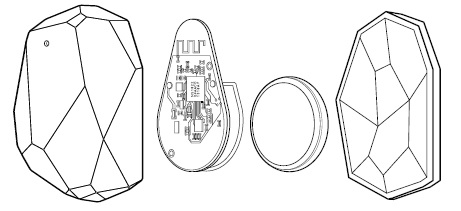
\includegraphics[width=0.6\textwidth]{images/estimotebeacon}
  \caption{Image of an Estimote beacon. Contains a small ARM processor, a Bluetooth Smart module and a battery, enclosed in silicone casing. Source: \protect\cite{ESTIMOTEBEACON}}
  \label{fig:estimotebeacon}
\end{figure}

The beacons broadcast signals. 
The beacons can broadcast these in an interval between \SI{100}{\milli\second} and \SI{2000}{\milli\second},
however an operating system such as iOS only scans for signals every \SI{1}{\second}.
Likewise, the beacons can broadcast the signals with a broadcasting power between \num{4} dBm and \num{-30}.
The further the signals travels, the weaker they get.
This means that the further away from a beacon you receive the signal, 
the weaker it is, and thus the accuracy falls. 
In short, the distance estimates will be more accurate the closer to a beacon you are. 

Estimote Beacons uses the iBeacon protocol. 
Each iBeacon packet include \cite{IBEACON}:
\begin{description}
  \item[UUID] A \SI{16}{\byte} identifier string 
  \item[Major] A \SI{2}{\byte} string to identify a subset of beacons within a larger group
  \item[Minor] A \SI{2}{\byte} string meant to identify individual beacons
  \item[Tx Power] A power defined as the signal exactly 1 meter from the device. This is used to estimate the distance between the devices. 
\end{description}

Estimote uses the iBeacon packets to estimate the distances. 
However, rather than trying to estimate exact distances, 
Estimote uses \emph{proximity zones}. 
There are four zones:
\begin{enumerate}
  \item Immediate (very close to the beacon)
  \item Near (about 1-3 meters from the beacon)
  \item Far (further away or the signal is fluctuating too much to make a better estimate)
  \item Unknown 
\end{enumerate}

By using \num{3} or more beacons, it is possible to estimate the users location. 
A typical method of estimating the location is trilateration. 
However, Estimote found that this method could not get better accuracy than \SI{5}{\meter}.
To get better results, 
they utilize particle filtering, sensor fusion and noise reduction algorithms.

\subsubsection{Indoor Location with Estimote}
Estimote, aside from offering the typical use case for beacons like entering a specific region, 
has also specialized in indoor location of users using the iBeacon protocol. 
The company has developed and released the Estimote Indoor Location SDK\footnote{https://github.com/Estimote/iOS-Indoor-SDK}.
They have also released a demo application for iOS\footnote{https://itunes.apple.com/us/app/estimote-indoor-location/id963704810}, 
which is meant to ease configuration needed for indoor location. 

A user will install the beacons in a room by placing a minimum of \num{4} beacons on the walls, 
preferably in the middle of each wall in a rectangular room.   
Next the user walks along the perimeter of the room, 
and thereby registering the location of the beacons, 
by collecting signal strengths from the beacons (a feature of the iBeacon protocol), 
and data from the phones accelerometer and/or gyroscope.
After the configuration, the application will have estimated the length of and placement of the walls, 
along with the signal strengths of each beacon.

To analyze the precision, 
to see whether we could actually use these beacons and Estimote's SDK, 
we performed a few tests. 
During our tests we found that the approach for configuring the indoor positioning, 
as described above, works terribly or not at all. 
After configuring the room, 
the application would show an illustration of the registered room, 
and we found the measurements to to be very inaccurate.
We have decided not to use the built-in room configuration. 
\todo[author=Thalley]{Indsæt nogle beskrivende tal eller illustrationer til at forklare hvor ringe det faktisk var}

\subsubsection{Configuring Rooms Programmatically}
As mentioned, Estimote provides the Estimote Indoor Location SDK, 
for performing indoor positioning using beacons on iOS. 
The SDK provides two mechanisms for configuring a room for indoor positioning.

\begin{enumerate}
\item Using the built-in controller. The component presents the user with a guided configuration similar to the one used in the Estimote Indoor Location application.
\item Programmatically using the \texttt{ESTLocationBuilder} class.
\end{enumerate}

The built-in controller was abandoned as it resulted in poor accuracy.

The \texttt{ESTLocationBuilder} lets developers configure a room programmatically, 
by passing coordinates (\texttt{ESTPoint}s) and an orientation to the builder. 
The $X$ and $Y$ value of each coordinate is measured in meters. 
Therefore a set of coordinates $\{(0, 0), (0, 5)\}$ represents a horizontal line of $5$ meters, 
and the set of coordinates $\{(0,0),(0,5),(5,5),(5,0)\}$ represents $5$ by $5$ meter room.

\Cref{fig:estlocationbuilder-livingroom} shows an example of a location created programmatically using the \texttt{ESTLocationBuilder}. The room is created using the following set of coordinates: $\{(0, 0), (5.37, 0), (5.37, 0.6), (6.9, 0.6), (6.9, 3.85), (0, 3.85)\}$.

\begin{figure}[!htb]
  \centering
  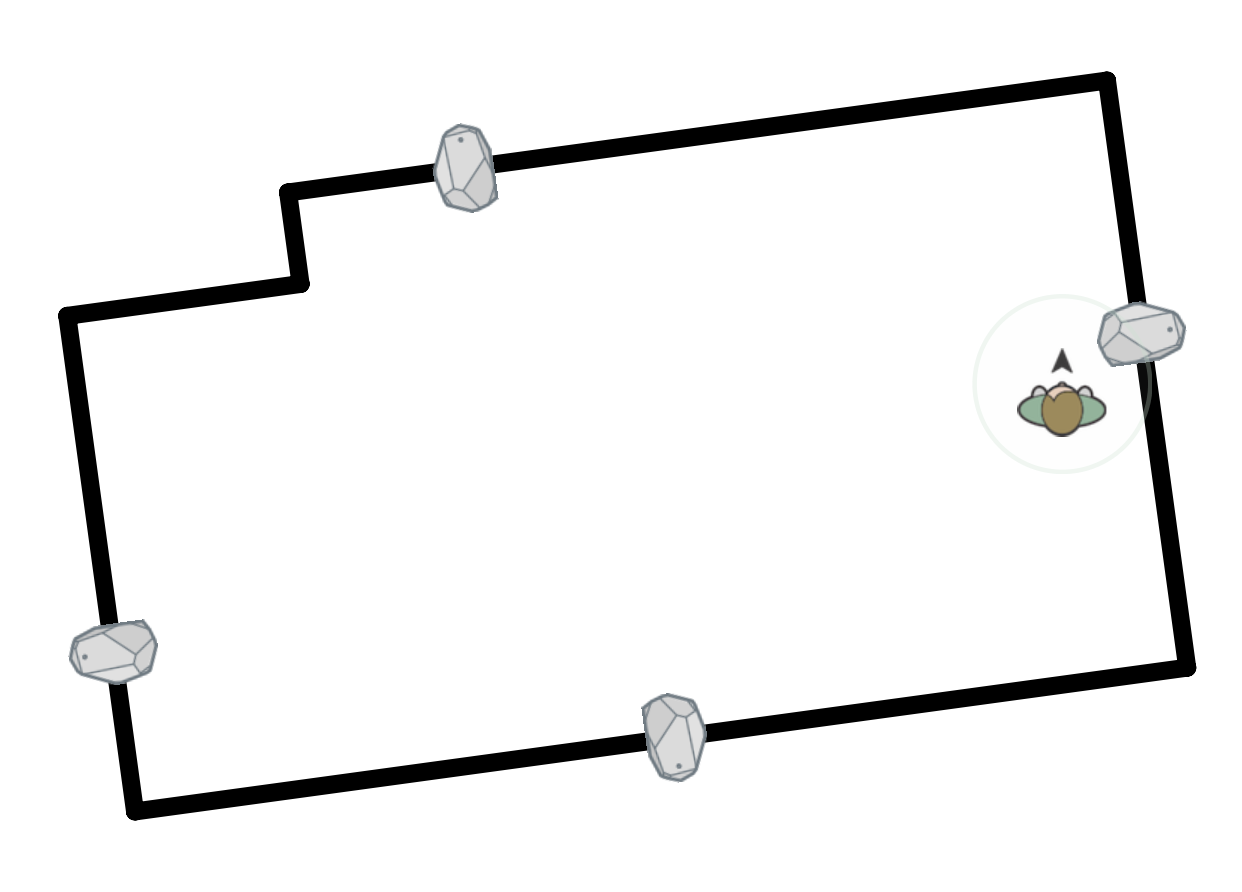
\includegraphics[width=0.33\textwidth]{images/living-room}
  \caption{Location created using the \texttt{ESTLocationBuilder}. Note that the model is rotated accordingly to the orientation of the room and the position of north relative to the user.}
  \label{fig:estlocationbuilder-livingroom}
\end{figure}

The builder is configured with $6$ coordinates that gives information about the shape of the room. 
Next, the beacons are added to the walls of the room. 
Beacons are added with the identifier of the beacon, 
such as \texttt{dec18deac0c5} for the \texttt{ice3} beacon. 
Lastly the orientation of the room relative to north and the name of the room is set. 
When the room has been configured, 
it can be stored on the users Estimote account using the Estimote SDK.
Using the \texttt{ESTLocationBuilder} to model a room reduces any uncertainties in estimating the users location, 
caused by an imprecise model of the room.

%%% Local Variables:
%%% mode: latex
%%% TeX-master: "../../master"
%%% TeX-command-extra-options: "-shell-escape"
%%% End:


%%% Local Variables:
%%% mode: latex
%%% TeX-master: "../../master"
%%% TeX-command-extra-options: "-shell-escape"
%%% End:
